%======================================================================
\chapter{Liquid-Filled HCPCF}
%======================================================================
\section{Filling Methods}
Fibers were cut to between 6cm and 8cm in length. To ensure consistent coupling and positioning, light was coupled to the core of the fiber by connecting to a solid-core PM780HP fiber via a mechanical splicing chip \cite{maruf}. We replaced the air in 1550nm HCPCF with deionized water and heavy water by utilizing capillary action. To selectively fill the core of 800nm HCPCF, the photonic crystal cladding was collapsed while leaving the hollow-core open and is similarly filled with liquid using capillary action. We collapsed the cladding by placing the HCPCF opposite of a solid-core fiber in a fusion splicer \cite{xiao} and adjusting arc current duration and power to melt the cladding structure while remaining distanced enough to prevent fusion with the solid-core fiber. 
\begin{figure}[!htb]
	\centering
	\foreach \x in {50ms 15mA, 70ms 20mA, 70ms 25mA, 80ms 25mA, 90ms 25mA, 100ms 25mA}
	{ 
	\begin{subfigure}[b]{0.3\textwidth}
		\includegraphics[width=\textwidth]{./Figures/fiberfilling/arc_power/\x.png}
		\caption{\x}
	\end{subfigure}
	\hfil
	}
	\caption{Side profile of collapsed cladding 1550HC fiber running the fiber splicer with varying current strength and duration. }
	\label{fig:selective filling}
\end{figure}
\begin{figure}[!htb]
	\centering
	\foreach \x in {collapsed, fiberend}
	{ 
	\begin{subfigure}[b]{0.4\textwidth}
		\includegraphics[width=\textwidth]{./Figures/fiberfilling/arc_err/\x.jpg}
	\end{subfigure}
	\hfil
	}
	\caption{Variation between fibers using splicer settings 70ms 25ms  }
	\label{fig:selective err}
\end{figure}
\clearpage

\section{Experimental Set-Up}
\begin{figure}[!htb]
	\centering
	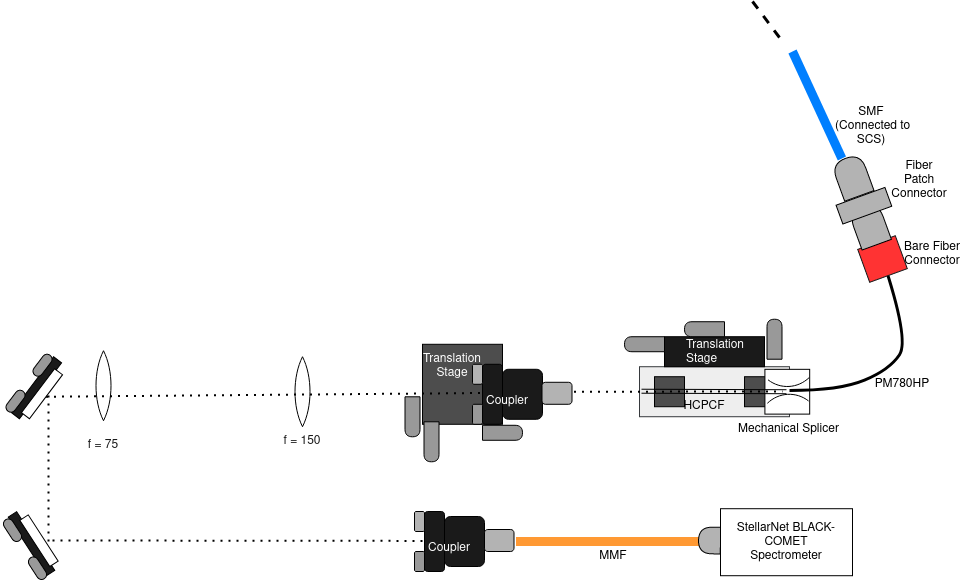
\includegraphics[width=0.75\textwidth]{./Figures/fiberfilling/scs_setup.png}
	\caption{Fiber transmission experimental set-up.}
	\label{fig:filling exp}
\end{figure}


\section{H${}_2$O and D${}_2$O Transmission}
HCPCF uses a photonic crystal cladding composed of a periodic silica structure that allows light to be guided through
a hollow and thus low-refractive index core. In some applications of HCPCF, such as fiber-integrated sensors and
on-linear optics, the hollow regions of the fiber are filled with liquids or gasses. Fibers that are fully-filled with water will  produce a frequency shift in the bandgap due to refractive index scaling\cite{antonopoulos}. On the other hand, when the core is selectively filled with water, light will be guided via total-internal reflection. We investigate the transmission spectra of fully-filled and core-filled fibers for deionized water and heavy water.
\begin{figure}[!htb]
	\centering
	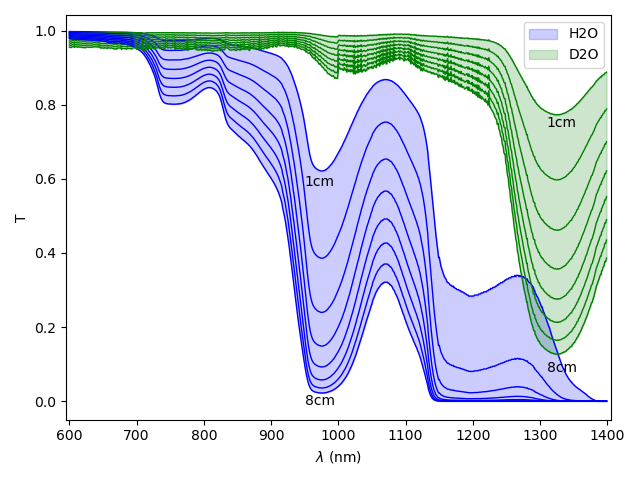
\includegraphics[width=0.7\textwidth]{./Figures/fiberfilling/water_transmission/water_transmission.png}
	\caption{The transmission of heavy water(green) and regular water(blue) is shown for slabs of thickness ranging from 1cm to 8cm in increments of 1cm using absorption data recorded by \cite{kedenburg}. }
	\label{fig:water transmission}
\end{figure}
\clearpage

\section{Results}
The air-filled 800nm HCPCF covers a transmission spectral range of 750nm–950nm. Light exits the fiber with a Gaussian mode shape and has an expected coupling between 75-80\% when connected to a solid-core single-mode fiber. A water-filled core retains a Gaussian mode shape and has a 30\% reduction in the normalized transmission for wavelengths above 850nm, which is consistent with the absorption spectrum of H2O \cite{kedenburg}. We also observe that the coupling efficiency of the fiber drops to 31\%. With a heavy water filled core, there are no significant changes in the normalized transmission spectrum, minimal effects to the absorption over this region, and coupling efficiency of up to 67\%.

The air-filled 1550nm HCPCF covers a transmission spectral range of 1200nm–1700nm. With a filled core and cladding, the spectral range shifts to transmitting wavelengths between 600nm–1100nm for both heavy water and water, which aligns with the scaling laws prediction. Heavy water achieved a coupling efficiency of 47\%, but water only 16\%. The existing mode shape is roughly Gaussian but contains noise as some light also leaks from the photonic structure, worse for water than heavy water. The losses seen in water are not entirely explained, but losses and effects from the decrease in refractive index contrast are also present in the D2O-filled fiber. While there is a less than 20\% difference in absorption coefficient between the 550nm–830nm for the fiber length, 7.6nm, between 830nm–950nm the absorption coefficient of water increases steeply but stays constant over the same region for heavy water. 
\subsection{Selective Filling}
\begin{figure}[!htb]
	\centering
	\includegraphics[width=0.75\textwidth]{./Figures/fiberfilling/HC800/transmission.png}
	\caption{Transmission of H${}_2$O and D${}_2$O in (a)selectively-filled 800nm hollow-core fiber.}
	\label{fig:trans 800hc}
\end{figure}
\clearpage

\subsection{Full-Fiber Filling}
\begin{figure}[!htb]
	\centering
	\foreach \x in {HC1550_empty, HC1550_full_D2O, HC1550_H2O}
	{ 
		\begin{subfigure}[b]{0.32\textwidth}
			\includegraphics[width=\textwidth]{./Figures/fiberfilling/HC1550/ModeShape/\x.png}
			\caption{}
	\end{subfigure}
		\hfil
	}
	\caption{Modeshape of 1550 hollow-core fiber filled with (a)air (b)heavy water (c)distilled water. Fiber filled with heavy water maintains a Gaussian profile while the fiber with regular distilled water shows some distortion.}
	\label{fig:1550 modeshape}
\end{figure}

\begin{figure}[!htb]
	\centering
	\includegraphics[width=0.75\textwidth]{./Figures/fiberfilling/HC1550/transmission.png}
	\caption{Transmission of H${}_2$O and D${}_2$O in fully-filed 1550nm hollow-core fiber.}
	\label{fig: trans 1550hc}
\end{figure}
\clearpage

\begin{thebibliography}{fiberfilling}
\bibitem{antonopoulos} G. Antonopoulos, F. Benabid, T. A. Birks, D. M. Bird, J. C. Knight, and
P. St. J. Russell, “Experimental demonstration of the frequency shift of
bandgaps in photonic crystal fibers due to refractive index scaling,” Opt.
Express, vol. 14, no. 7, p. 3000, 2006.

\bibitem{maruf} R. A. Maruf and M. Bajcsy, “On-chip splicer for coupling light between
photonic crystal and solid-core fibers,” Appl. Opt., vol. 56, no. 16, p.
4680, Jun. 2017.

\bibitem{xiao} L. Xiao, W. Jin, M. S. Demokan, H. L. Ho, Y. L. Hoo, and C. Zhao,
“Fabrication of selective injection microstructured optical fibers with a
conventional fusion splicer,” Opt. Express, vol. 13, no. 22, p. 9014, 2005.

\bibitem{kedenburg} S. Kedenburg, M. Vieweg, T. Gissibl, and H. Giessen, “Linear refractive
 index and absorption measurements of nonlinear optical liquids in the
 visible and near-infrared spectral region,” Opt. Mater. Express, vol. 2,
no. 11, p. 1588, Nov. 201
\end{thebibliography}